\documentclass[fleqn,10pt]{latex/stylish_article} % Document font size and equations flushed left

\setcounter{tocdepth}{3}

% Pandoc environments
\usepackage{framed}
\usepackage{fancyvrb}
\providecommand{\tightlist}{%
  \setlength{\itemsep}{0pt}\setlength{\parskip}{0pt}}
\newcommand{\VerbBar}{|}
\newcommand{\VERB}{\Verb[commandchars=\\\{\}]}
\DefineVerbatimEnvironment{Highlighting}{Verbatim}{commandchars=\\\{\}, fontsize=\scriptsize} % R Code

% Colored code
\usepackage{color}
\definecolor{shadecolor}{RGB}{248,248,248}
\newenvironment{Shaded}{\begin{snugshade}}{\end{snugshade}}
\newcommand{\KeywordTok}[1]{\textcolor[rgb]{0.13,0.29,0.53}{\textbf{{#1}}}}
\newcommand{\DataTypeTok}[1]{\textcolor[rgb]{0.13,0.29,0.53}{{#1}}}
\newcommand{\DecValTok}[1]{\textcolor[rgb]{0.00,0.00,0.81}{{#1}}}
\newcommand{\BaseNTok}[1]{\textcolor[rgb]{0.00,0.00,0.81}{{#1}}}
\newcommand{\FloatTok}[1]{\textcolor[rgb]{0.00,0.00,0.81}{{#1}}}
\newcommand{\ConstantTok}[1]{\textcolor[rgb]{0.00,0.00,0.00}{{#1}}}
\newcommand{\CharTok}[1]{\textcolor[rgb]{0.31,0.60,0.02}{{#1}}}
\newcommand{\SpecialCharTok}[1]{\textcolor[rgb]{0.00,0.00,0.00}{{#1}}}
\newcommand{\StringTok}[1]{\textcolor[rgb]{0.31,0.60,0.02}{{#1}}}
\newcommand{\VerbatimStringTok}[1]{\textcolor[rgb]{0.31,0.60,0.02}{{#1}}}
\newcommand{\SpecialStringTok}[1]{\textcolor[rgb]{0.31,0.60,0.02}{{#1}}}
\newcommand{\ImportTok}[1]{{#1}}
\newcommand{\CommentTok}[1]{\textcolor[rgb]{0.56,0.35,0.01}{\textit{{#1}}}}
\newcommand{\DocumentationTok}[1]{\textcolor[rgb]{0.56,0.35,0.01}{\textbf{\textit{{#1}}}}}
\newcommand{\AnnotationTok}[1]{\textcolor[rgb]{0.56,0.35,0.01}{\textbf{\textit{{#1}}}}}
\newcommand{\CommentVarTok}[1]{\textcolor[rgb]{0.56,0.35,0.01}{\textbf{\textit{{#1}}}}}
\newcommand{\OtherTok}[1]{\textcolor[rgb]{0.56,0.35,0.01}{{#1}}}
\newcommand{\FunctionTok}[1]{\textcolor[rgb]{0.00,0.00,0.00}{{#1}}}
\newcommand{\VariableTok}[1]{\textcolor[rgb]{0.00,0.00,0.00}{{#1}}}
\newcommand{\ControlFlowTok}[1]{\textcolor[rgb]{0.13,0.29,0.53}{\textbf{{#1}}}}
\newcommand{\OperatorTok}[1]{\textcolor[rgb]{0.81,0.36,0.00}{\textbf{{#1}}}}
\newcommand{\BuiltInTok}[1]{{#1}}
\newcommand{\ExtensionTok}[1]{{#1}}
\newcommand{\PreprocessorTok}[1]{\textcolor[rgb]{0.56,0.35,0.01}{\textit{{#1}}}}
\newcommand{\AttributeTok}[1]{\textcolor[rgb]{0.77,0.63,0.00}{{#1}}}
\newcommand{\RegionMarkerTok}[1]{{#1}}
\newcommand{\InformationTok}[1]{\textcolor[rgb]{0.56,0.35,0.01}{\textbf{\textit{{#1}}}}}
\newcommand{\WarningTok}[1]{\textcolor[rgb]{0.56,0.35,0.01}{\textbf{\textit{{#1}}}}}
\newcommand{\AlertTok}[1]{\textcolor[rgb]{0.94,0.16,0.16}{{#1}}}
\newcommand{\ErrorTok}[1]{\textcolor[rgb]{0.64,0.00,0.00}{\textbf{{#1}}}}
\newcommand{\NormalTok}[1]{{#1}}

% cslreferences environment required by pandoc > 2.7

% Polyglossia
\usepackage{polyglossia}
\setmainlanguage{en-US}

% Figures
\usepackage{graphicx,grffile}
\makeatletter
\def\maxwidth{\ifdim\Gin@nat@width>\linewidth\linewidth\else\Gin@nat@width\fi}
\def\maxheight{\ifdim\Gin@nat@height>\textheight0.8\textheight\else\Gin@nat@height\fi}
\makeatother
% Scale images if necessary, so that they will not overflow the page
% margins by default, and it is still possible to overwrite the defaults
% using explicit options in \includegraphics[width, height, ...]{}
\setkeys{Gin}{width=\maxwidth,height=\maxheight,keepaspectratio}

% Additional packages
\RequirePackage{natbib}             % Advanced Bibliography (citep...).
\RequirePackage{amsmath,amsfonts,amssymb}
\RequirePackage{breqn}              % Line breaks in equations
\RequirePackage{url}                % Line breaks in url's
\RequirePackage{enumitem}           % Line spacing in lists
  \setlist[itemize]{noitemsep,nolistsep}
  \setlist[enumerate]{noitemsep,nolistsep}

% Tables
\usepackage{longtable,booktabs}
\usepackage{caption}
% These lines are needed to make table captions work with longtable:
\makeatletter
\def\fnum@table{\tablename~\thetable}
\makeatother
% longtable 2 columns
% https://tex.stackexchange.com/questions/161431/how-to-solve-longtable-is-not-in-1-column-mode-error
\makeatletter
\let\oldlt\longtable
\let\endoldlt\endlongtable
\def\longtable{\@ifnextchar[\longtable@i \longtable@ii}
\def\longtable@i[#1]{\begin{figure}[t]
\onecolumn
\begin{minipage}{0.5\textwidth}\scriptsize
\oldlt[#1]
}
\def\longtable@ii{\begin{figure}[t]
\onecolumn
\begin{minipage}{0.5\textwidth}\scriptsize
\oldlt
}
\def\endlongtable{\endoldlt
\end{minipage}
\twocolumn
\end{figure}}
\makeatother

% Full-width tables
\usepackage{tabu}
\renewenvironment{table}{\begin{table*}}{\end{table*}\ignorespacesafterend}
  

% hyperref comes last
\RequirePackage{hyperref}           % Hypertext links, PDF bookmarks
  \hypersetup{urlcolor=blue,linkcolor=black,citecolor=black,colorlinks=true}

%----------------------------------------------------------------------------------------
%	ARTICLE INFORMATION
%----------------------------------------------------------------------------------------

\JournalInfo{Hal 01212435 v3} % Journal information
\Archive{\ }

\PaperTitle{Practical Estimation of Diversity from Abundance Data} % Article title

\Authors{
Eric Marcon\textsuperscript{1,2*}
} % Authors
\affiliation{
\textsuperscript{1}AgroParisTech, AMAP, CIRAD, CNRS, INRAE, IRD, Univ Montpellier, Montpellier, France.\\ \hspace{1em} \\\textsuperscript{2}UMR EcoFoG, AgroParisTech, CIRAD, CNRS, INRAE, Univ Antilles, Univ Guyane, Kourou, France.\\ \hspace{1em} 
}
\affiliation{*\textbf{Corresponding author}: \href{mailto:eric.marcon@agroparistech.fr}{\nolinkurl{eric.marcon@agroparistech.fr}}, } % Corresponding author

\Keywords{biodiversity, entropy, estimation} % Keywords
\newcommand{\keywordname}{Keywords} % Defines the keywords heading name

%----------------------------------------------------------------------------------------
%	ABSTRACT
%----------------------------------------------------------------------------------------

\Abstract{
Measuring biodiversity requires empirical techniques to effectively estimate it from real data. The well-known underestimation of the number of species applies to low orders of diversity in general. I test nine estimators including three new ones on geometric and lognormal distributions that represent realistic, hyper-diverse communities. The best two estimators allow a good estimation of diversity of orders over 0.5, even when the sampling effort is low. I provide criteria to choose the estimator and the necessary code in the R package entropart.
}

%----------------------------------------------------------------------------------------

\begin{document}

\selectlanguage{en-US}

\flushbottom % Makes all text pages the same height

\maketitle % Print the title and abstract box

\tableofcontents % Print the contents section

\thispagestyle{empty} % Removes page numbering from the first page

%----------------------------------------------------------------------------------------
%	ARTICLE CONTENTS
%----------------------------------------------------------------------------------------

\hypertarget{introduction}{%
\section{Introduction}\label{introduction}}

Measuring biodiversity requires both a robust theoretical framework \citep{Patil1982} and empirical techniques to effectively estimate the theoretical variables with real data \citep{Beck2010}.
In this paper I focus on species-neutral measures of diversity based on HCDT entropy \citep{Havrda1967, Daroczy1970, Tsallis1988} that fulfill the first requirement.
Entropy measures the average surprise brought by observing individuals of a community.
Surprise is a decreasing function of probability dropping to 0 when probability is 1.
HCDT entropy uses a parameterized surprise function that is the deformed logarithm of order \(q\) of the reciprocal of probability \citep{Marcon2014a}.
Traditional measures of diversity, namely the number of species as well as Shannon's and Simpson's indices, are special cases of the HCDT entropy for values of \(q\) equal to 0, 1 and 2.
HCDT entropy should be transformed into Hill numbers \citep{Hill1973} for better interpretation of the value of diversity as an effective number of species \citep{Jost2006}.
Hill numbers are simply the deformed exponential of HCDT entropy \citep{Marcon2014a}.
Rather than focusing on a single value of \(q\), a profile of diversity, i.e.~a plot of diversity against \(q\), can be built \citep{Tothmeresz1995}.
Low values of \(q\) (starting from 0) give much importance to rare species, whilst higher values (usually up to 2) focus on abundant species.
Negative values of \(q\) are not used because of poor mathematical properties of their entropy \citep{Beck2009}, and values over 2 generally bring little more information.
Ordering communities in terms of diversity requires that their profile do not cross \citep{Tothmeresz1995}; else, declaring a community more diverse than another only holds for a range of values of \(q\) reflecting the importance given to rare or frequent species \citep{Lande2000}.

To plot those profiles, diversity must be estimated from the data.
Estimation bias \citep[following the terminology of][]{Dauby2012} is a well-known issue \citep{Marcon2014a}.
Real data are almost always samples of larger communities, so some species may have been missed.
The induced bias on the Simpson entropy is smaller than on the Shannon entropy because the former assigns lower weights to rare species, i.e.~the sampling bias is even more important when \(q\) decreases.
Another estimation bias has been widely studied by physicists who generally consider that all species of a given community are known and their probabilities quantified.
Their main issue is not at all missing species but the non-linearity of entropy measures \citep[see][ for a short review]{Bonachela2008}.
Estimating probabilities at power \(q>0\) by the power of their estimator is an important source of underestimation of entropy.
The need for corrections has generated a considerable literature in ecological statistics and statistical physics.

This paper tests the performance of the state-of-the-art estimators when applied to the kind of data ecologists have to deal with.
It starts with simulated distributions that have the advantage of being easily manipulated to generate various sampling intensities and evaluate the bias and root mean square error (RMSE) of the estimators.
The classical models of the literature, namely the lognormal and the geometric distributions are addressed.
The lognormal distribution describes, at least roughly, many hyper-diverse ecosystems even though the link between its statistical success and the underlying ecological mechanisms is poorly documented \citep{Tokeshi1993}.
The geometric distribution is a far more difficult case because it is very uneven: the frequency of rare species is several orders of magnitude smaller than that of the frequent ones, making it impossible to observe with reasonable sampling effort \citep{Haegeman2013}.
The best-known and best-performing estimators, including three new ones, are applied to those distributions and two actual forest data sets.
The purpose of the paper is to provide recommendations about the estimation technique to choose when facing different types of data and draw general conclusions about the possible accuracy of diversity estimation.

Phylogenetic entropy is the sum of HCDT entropy along an ultrametric tree \citep{Marcon2014b} so estimating it reduces to estimating HCDT entropy.
Phylogenetic diversity is then obtained as the deformed exponential of phyloentropy.
In short, estimating phylodiversity relies on the methods presented here so the paper will focus on species-neutral diversity for clarity.

All analyses are made whith the package \emph{entropart} \citep{Marcon2014c} for R \citep{R}.
This paper comes with a Shiny application available on GitHub \footnote{\url{https://github.com/EricMarcon/estimation}} to simulate communities and estimate their diversity.

\hypertarget{methods}{%
\section{Methods}\label{methods}}

Consider a community of species indexed by \(s=1,\ 2,\dots ,S\). \(n_{s}\) is the number of individuals of species \(s\) sampled in the community, \(n=\sum_s{n_{s}}\) the total number of sampled individuals.
The (unknown) probability \(p_{s}\) for an individual to belong to species \(s\) is estimated by \({\hat{p}}_{s}={n_{s}}/{n}\).
The number of species represented by \(\nu\) individuals in the sample of size \(n\) is \({s}^{n}_{\nu}\), so \({s}^{n}_{0}\) if the (unknown) number of unobserved species considering the sampling effort.
\({s}^{n}_{\nu}\) is considered as a realization of the random variable \({S}^{n}_{\nu}\) so it is used to estimate its expectation \({\mathbb E}({S}^{n}_{\nu})\).

\(\pi_\nu\) is the sum of the probabilities \(p_s\) of species represented by \(\nu\) individuals.

The deformed logarithm formalism \citep{Tsallis1994} is very convenient to manipulate entropies.
The deformed logarithm of order \(q\) is defined as:

\begin{equation}
  \ln_q{x}=\frac{x^{1-q}-1}{1-q}
  \label{eq:lnq}
\end{equation}

It converges to the natural logarithm when \(q\to 1\).

The inverse function of \(\ln_q{x}\) is the deformed exponential:

\begin{equation}
  e^x_q=[1+(1-q)x]^{\frac{1}{1-q}}
  \label{eq:expq}
\end{equation}

\hypertarget{sample-coverage}{%
\subsection{Sample coverage}\label{sample-coverage}}

The sample coverage \citep{Good1953} is the probability for an individual in the community to belong to a species observed in the sample.
It equals the sums of the probabilities of the observed species.
It is an essential tool for diversity estimation because it is included in some estimators, e.g. \citet{Chao2003}, and it allows the evaluation of the completeness of the sampling \citep{Chao2012b}.
Its estimator given by Good is:

\begin{equation}
    \hat{C} = 1-\frac{{s}^{n}_{1}}{n}
  \label{eq:CGood}
\end{equation}

It is biased \citep{Zhang2007}, because:

\begin{equation}
  C = 1-\frac{{\mathbb E}({S}^{n}_{1}) - \pi_1}{n}
  \label{eq:CsansBiais}
\end{equation}

Good's estimator neglects the term \(\pi_1\), the sum of the probabilities of singletons.
It was built from Turing's frequency formula relating the average probability of species observed \(\nu\) times to the number of species observed \(\nu+1\) and \(\nu\) times.
This formula has been improved by Chao \emph{et al.} \citep{Chao2010a, Chiu2014a} to estimate \(\pi_1\).
Estimating the number of species by the Chao1 estimator \citep{Chao1984}, \citet{Chao2010a} obtained an improved estimator of the sample coverage:

\begin{equation} 
    \hat{C} = 1-\frac{{s}^{n}_{1}}{n}\left[\frac{\left(n-1\right){s}^{n}_{1}}{\left(n-1\right){s}^{n}_{1}+2{s}^{n}_{2}{}}\right]
  \label{eq:CChao}
\end{equation}

This estimator has been further used by \citet{Chao2015} to derive an estimator of entropy (see below).

An almost unbiased estimator has been derived using the information provided by the whole distribution \citep{Chao1988, Zhang2007}:

\begin{equation}
  \hat{C}=1-\sum^{n}_{\nu=1}{\left(-1\right)}^{\nu+1}{\binom{n}{\nu}}^{-1}{s}^{n}_{\nu}
  \label{eq:CZhang}
\end{equation}

It is used in this paper.

\hypertarget{estimators-of-entropy}{%
\subsection{Estimators of entropy}\label{estimators-of-entropy}}

The existing estimators and the new ones proposed here can be classified into four main methods.
The simplest one just consists of plugging the estimator of \(p_s\), i.e.~\(\hat{p}_s = n_s/n\), into the definition of diversity to evaluate to obtain a so-called plug-in estimator, sometimes named naive estimator.
The plug-in estimator of HCDT entropy of order \(q\) is:

\begin{equation}
  ^{q}{\hat{H}} = \sum_{s}{{\hat{p}}_s \ln_q{\frac{1}{\hat{p}}_s}}
  \label{eq:Hplugin}
\end{equation}

The plug-in estimator is useless in hyper-diverse communities because it severely underestimates diversity because of unobserved species and of the non-linearity of estimators.

Recent progress has been made in estimating the actual distribution of the probability of species by fitting a model of their distribution to the data.
The distribution of the unobserved species can be added if their number is estimated and a distribution form is chosen.
\citet{Chao2014c} used a two-parameter model based on the estimation of the generalized sample coverage (not detailed here), estimated the total richness with the Chao1 estimator and modeled the unobserved species as a geometric distribution to unveil the complete rank-abundance distribution of an observed community.
They applied the plug-in estimator this distribution: It will be called the ``Chao-unveiled'' here.

The Chao1 estimator was built according to the same theoretical approach as that of the unveiled rank-abundance distribution.
It is a lower-bound estimator of the number of species.
It has been improved by \citet{Chiu2014a} who slightly reduced its negative bias with the iChao1 estimator, integrating species represented by 3 and 4 individuals.
The ``iChao-unveiled'' estimator will be defined here as a variation on the ``Chao-unveiled'' estimator, where richness is estimated by the iChao1 estimator.

The jackknife estimator \citep{Burnham1979} has shown good performances to estimate richness when the sampling effort is too low for the Chao1 estimator to perform well \citep{Brose2003} even though it actually lacks theoretical support \citep{Cormack1989}.
Estimating species richness with the jackknife estimator, whose order is selected according to the data, defines the ``jackknife-unveiled'' estimator.
Using the jackknife estimator to unveil the tail of the abundance distribution was not the intention of \citet{Chao2014c} because it is not consistent with their theoretical framework.
It must be seen here as a merely empirical tool.

The second method relies on the \citet{Horvitz1952} estimator of the weighted sum of a function of its elements \({x_1, x_2, ..., x_S}\), say \(\sum_{s}{p_s f(x_s)}\) when some of them are not observed.
An unbiased estimator of the sum is obtained when each term is divided by its probability to be observed \(1-(1-p_s)^n\).
\citet{Chao2003} proposed to combine it with the estimator of the sample coverage: conditionally to the set of observed species, an unbiased estimator \citep{Ashbridge2000} of \(p_s\) is \(\tilde{p}_s = \hat{C} \hat{p}_s\).
Chao and Shen estimated the Shannon entropy; the method has then been extended to HCDT entropy \citep{Marcon2014a} and similarity-based diversity \citep{Marcon2014e}:

\begin{equation}
  ^{q}{\tilde{H}} =\sum_{s}{\frac{\hat{C}{\hat{p}}_s\ln_q\dfrac{1}{\hat{C}{\hat{p}}_s}}{1-{\left(1-\hat{C}{\hat{p}}_s\right)}^n}}
\end{equation}

A further progress can be done by replacing the conditional estimator of probabilities \(\tilde{p}_s = \hat{C} \hat{p}_s\) by that of \citet{Chao2014c}.
Since the improved probability estimator depends on the generalized sample coverage, the improved Chao-Shen estimator will be named the ``generalized coverage'' estimator.

The third method has been derived by \citet{Grassberger1988} who gave a reduced-bias estimator of the value of an integer at power \(q\).
\({p_s^q}\) is written as \(n_s^q/n^q\) and \(n_s^q\) is estimated \citep{Marcon2014a} as:

\begin{equation}
  \tilde{n}^{q}_{s}
  = \frac{\mathrm{\Gamma}\left(n_s +1\right)}{\mathrm{\Gamma}\left(n_s -q+1\right)}
  + \frac{{\left(-1\right)}^n \mathrm{\Gamma}\left(1+q\right)\sin{\pi q}}{\pi\left(n+1\right)}
\end{equation}

The estimator of \({p_s^q}\) is simply \(\tilde{p}^{q}_{s} = \tilde{n}^{q}_{s}/n^q\).
It is plugged into the formula of entropy to obtain the Grassberger estimator:

\begin{equation}
  ^{q}{\tilde{H}}
  = \frac{1-\sum_{s}{\tilde{p}^{q}_{s}}}{q-1}
  \label{eq:Grassberger}
\end{equation}

The last method has been the subject of an important literature in the last ten years.
A review can be found in \citet{Chao2013}, Appendix A.
It relies on the estimation of \(h_q=\sum_{s}{p_s^q}\).
\(h_q\) can be written as the following sum:
\begin{equation}
    h_q = \sum_{r=0}^{\infty}{\binom{q-1}{r} \left( -1\right)^r \zeta_r}
  \label{eq:hq}
\end{equation}

\(\zeta_r\) is the generalized Simpson entropy \(\sum_{s}{p_s(1-p_s)^r}\) defined by \citet{Zhang2010}.
The first \(n\) elements of the sum, denoted \(\tilde{h}_{q}\), can be estimated with no bias \citep{Zhang2014}:

\begin{equation}
  \tilde{h}_{q} = \sum_{s=1}^{S}{{\hat{p}}_{s}
      \sum_{v=1}^{n-n_s}{\left[ 
        \prod_{i=1}^{v}{\frac{i-q}{i} \prod_{j=1}^{v}{\left( 1-\frac{n_s-1}{n-j}\right) }} 
        \right] }}
\end{equation}

\citet{Zhang2013a} shows that the bias due to ignoring the remaining terms is asymptotically normal and decays exponentially fast.
I'll call the \citet{Zhang2014} estimator the one based on \(\tilde{h}_{q}\):

\begin{equation}
  ^{q}{\tilde{H}} = \frac{1-\tilde{h}_{q}}{q-1}
  \label{eq:Zhang2014}
\end{equation}

Some attempts have been made to estimate the remaining bias \citep{Zhang2013}.
The most achieved one is that of \citet{Chao2015}, completing \citet{Chao2013}.
It relies on the estimation of the total number of species by the Chao1 estimator and a few approximations including that the actual probabilities of unobserved species can be assumed almost equal.
A consequence is that the estimator of the average probability of species sampled once also equals the probability estimator of unobserved species.
Its value is noted \(A\).
It is \(2 {s}^{n}_{2} / {\left[\left( n-1 \right) {s}^{n}_{1} +2 {s}^{n}_{2} \right]}\) if singletons and doubletons are present or \(2/{\left[\left(n-1\right)\left({s}^{n}_{1} -1\right)+2\right]}\) if doubletons are missing.
The Chao-Jost estimator of HCDT entropy is:

\begin{multline}
  ^{q}{\tilde{H}}
    = \frac{1}{q-1} [ 1 -\tilde{h}_q \\
    -\frac{{s}^{n}_{1}}{n} {\left( 1-A \right)}^{1-n} \left( A^{q-1} -\sum^{n-1}_{r=0}{\binom{q-1}{r} {\left(A-1\right)}^r} \right) ]
\end{multline}

In absence of singletons and doubletons, \(A\) is set to 1 and the estimator is identical to that of Zhang and Grabchak.

\hypertarget{confidence-intervals}{%
\subsection{Confidence intervals}\label{confidence-intervals}}

Two methods allow the evaluation of confidence intervals: asymptotic, closed forms are available for some estimators, or bootstrapping is required in the general case.

\citet{Esty1983}, completed by \citet{Zhang2007}, showed that the estimator of sample coverage (eq. \eqref{eq:CZhang} is asymptotically normal with the following confidence interval:

\begin{equation}
    C=\hat{C}\pm t^{n}_{1-\alpha/2} \frac{\sqrt{{s}^{n}_{1}\left(1-\frac{{s}^{n}_{1}}{n}\right)+2{s}^{n}_{2}}}{n} 
\end{equation}

Where \(t^{n}_{1-\alpha/2}\) is the quantile of a Student distribution with \(n\) degrees of freedom at the risk threshold \(\alpha\), here 1.96 for all sample sizes and \(\alpha=5\%\).

The Zhang-Grabchak estimator is also asymptotically normal and comes with an asymptotic confidence interval \citep{Zhang2014} implemented in the package \emph{EntropyEstimation} \citep{Cao2014}.

The theoretical distribution of other estimators is unknown.
They must be built by bootstrap techniques: the observed community is re-sampled, say 1000 times, and entropy is calculated each time.
The \(\alpha/2\) and \(1-\alpha/2\) quantiles of the distribution of entropy are the bounds of the confidence interval.
The issue of re-sampling a community is the same as that of sampling it: rare species are often eliminated, so the entropy is underestimated.
Starting from the whole community, a first estimation bias is caused by sampling it.
The estimators presented here aim at correcting it.
When this observed community is re-sampled, a second estimation bias appears.
Estimating the entropy of re-sampled communities with bias correction yields, on average, the entropy of the observed community estimated by the plug-in estimator \citep{Marcon2012a}: if the estimator works well, it eliminates the second estimation bias but it cannot address the first one.
The solution to this problem is simply to recenter the entropy distribution of re-sampled communities around the value of the entropy of the observed community \citep{Marcon2012a, Chao2015}.

The re-sampling technique may just consist of drawing individuals in the observed community with replacement, or, equivalently, drawing a community in a multinomial distribution respecting the size and probability distribution of the observed community \citep{Marcon2014a}.
A more sophisticated technique has been proposed by \citet{Chao2015}.
Given the sample size, the probability distribution of observed species can be estimated more accurately than by the estimator \(\tilde{p}_s = \hat{C} \hat{p}_s\) which underestimates the probability of rare species \citep{Chao2014c}.
A better estimate of the probabilities is used (actually, a simplified version of that of the unveiled estimators above) and completed by an estimation of the number of unobserved species, whose probabilities are assumed identical.
Despite these extra efforts, the distribution of the entropy of re-sampled community still has to be recentered.

The confidence interval of a biased estimator must be understood as the variability of its results.
Since its bias is unknown, there is no guarantee that it contains the real value of diversity.

\hypertarget{from-entropy-to-diversity}{%
\subsection{From entropy to diversity}\label{from-entropy-to-diversity}}

All entropy estimations are finally transformed into diversity values to be interpretable \citep{Jost2006}.
It is not correct to recenter the confidence interval of diversity estimations because of the non-linearity of the transformation of entropy into diversity \citep{Marcon2012a}.
The correct process consists of evaluating entropy with its confidence interval and make the final exponential transformation of all values into diversity.

\hypertarget{typical-distributions}{%
\subsection{Typical distributions}\label{typical-distributions}}

\scriptsize

\normalsize

\scriptsize

\normalsize

Comparing the performance of estimators requires simulations of realistic communities.
The focus is put on two opposed models making sense in ecology.
The lognormal distribution \citep{Preston1948} fits well species-rich communities for several reasons, including populations dynamics \citep{Engen1996}, niche apportionment \citep{Bulmer1974}, or even statistical physics arguments \citep{Pueyo2007, Dewar2008}.
It is often well fitted empirically \citep{Tokeshi1990} even though it has been questioned theoretically \citep{Williamson2005}.
The local community distribution according to the neutral theory \citep{Volkov2003} is not lognormal but departs from it very moderately.
The logarithm of the species probabilities follows a Gaussian distribution.

The geometric series model \citep{Motomura1932, Whittaker1972} generates far more uneven species distributions.
In this model, the first species is represented by a part \(p\) of the total resources.
The second one has the same part \(p\) of the remaining resources, and so on.
Finally, probabilities are normalized to be proportional to the resources taken.



\scriptsize

\begin{figure}

{\centering 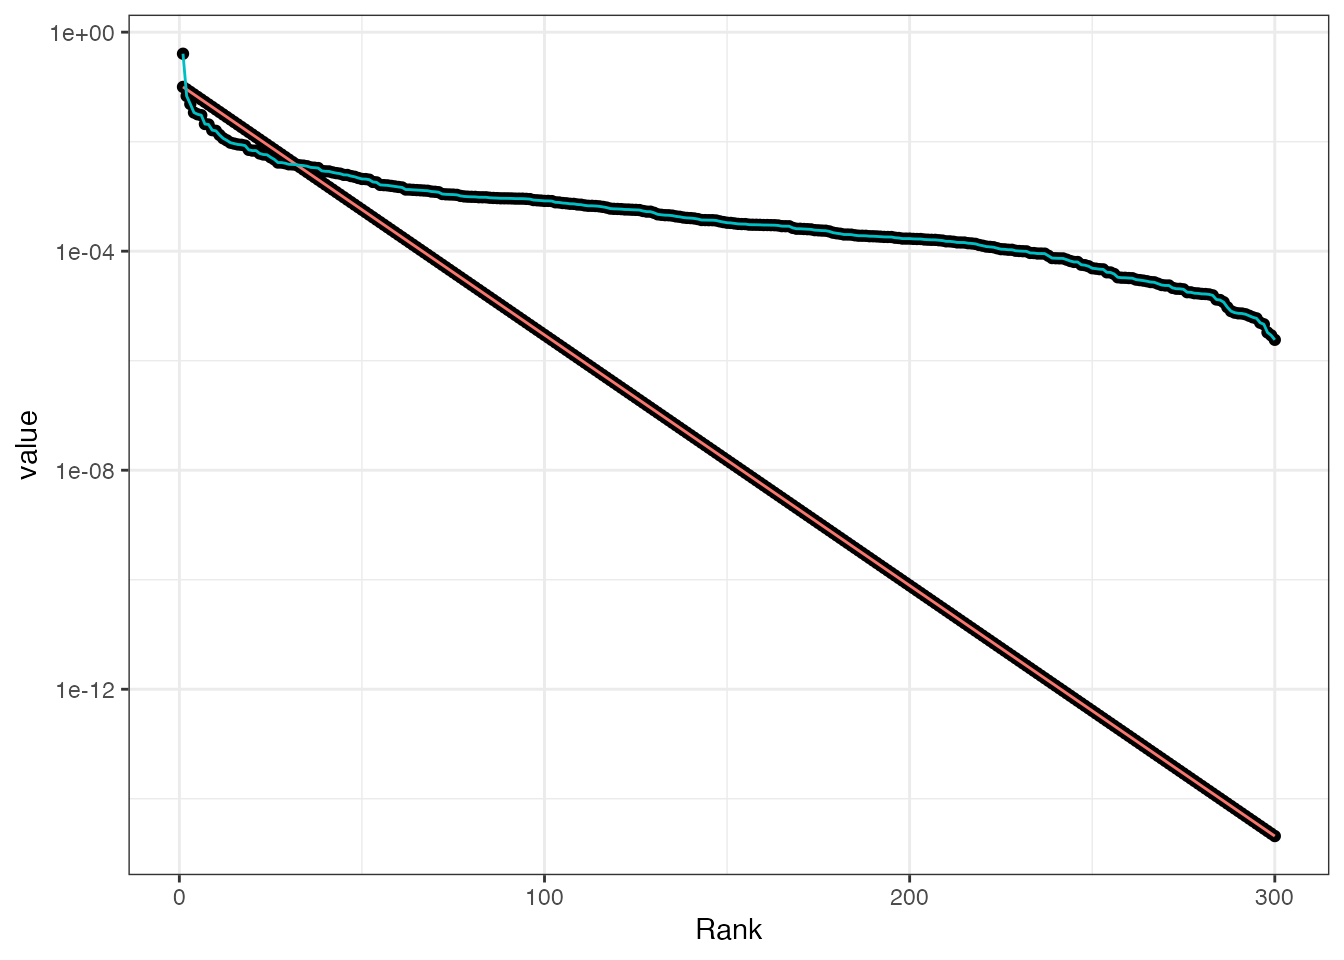
\includegraphics[width=0.8\linewidth]{PracticalEstimation_files/figure-latex/SpeciesDistributions-1} 

}

\caption{Rank-Abundance curves of 300 species following a lognormal (green, top curve) or a geometric distribution (red, straight line). The solid lines are the fitted models.}\label{fig:SpeciesDistributions}
\end{figure}

\normalsize

Artificial communities following those distributions are generated.
Figure \ref{fig:SpeciesDistributions} presents a lognormal one, with log-standard-deviation equal to 2 (typical of the distribution of tree species in a rainforest) and a geometric distribution with parameter \(p=0.1\).
Both contain 300 species.

\hypertarget{evaluation-of-the-performance-of-estimators}{%
\subsection{Evaluation of the performance of estimators}\label{evaluation-of-the-performance-of-estimators}}

The performance of each estimator was calculated as its average relative bias on all values of \(q\) (i.e.~the average difference between the mean simulated entropy and its true value) and it Root Mean Square Error (RMSE, i.e.~the square root of the sum of the squared bias and the variance, divided by the true value).
The true entropy of each reference distribution was calculated with the known values of \(p_s\).
For each reference distribution, 1000 random samples of the chosen size were drawn in a multinomial distribution respecting the reference probabilities \(p_s\).
Entropy was calculated for \(q\) between 0 and 2.
The average entropy and its first and last 2.5\% quantiles were retained to build the profile and its confidence envelope (which is quite different from that of the estimation of real communities).
Finally, entropy was transformed into diversity to be plotted.

\hypertarget{results}{%
\section{Results}\label{results}}

Simulations of independent sampling of individuals in real communities are multinomial samples of various sizes in the chosen species distributions.
Sample sizes are between 200 and 5000 individuals to cover a range from obvious undersampling to a high-effort inventory: 5000 individuals correspond to 9 to 10 ha of forest.

\hypertarget{sample-coverage-1}{%
\subsection{Sample coverage}\label{sample-coverage-1}}



\scriptsize

\begin{figure*}

{\centering 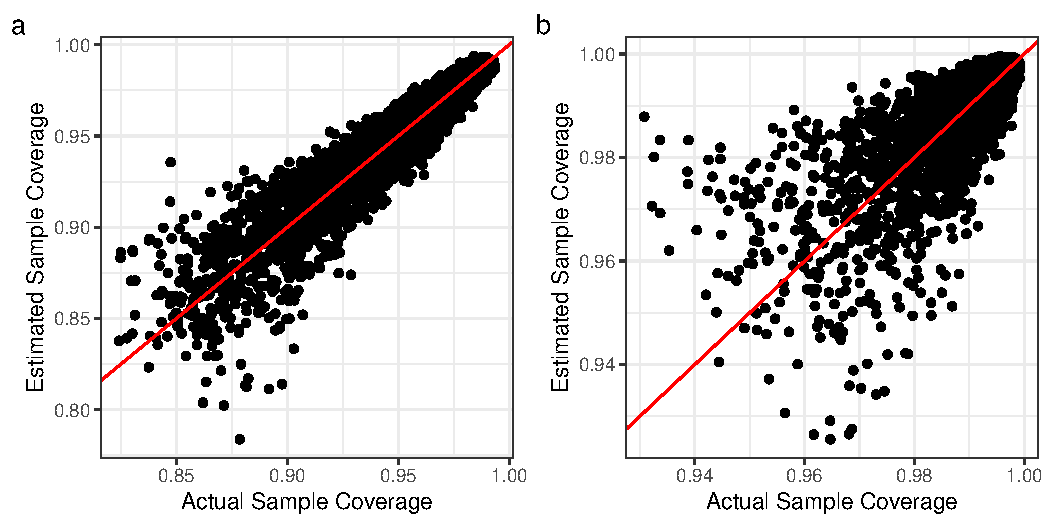
\includegraphics[width=0.8\linewidth]{PracticalEstimation_files/figure-latex/CAll-1} 

}

\caption{Estimated vs real sample coverage of simulated samples of a lognormal (a) or geometric (b) distribution of 300 species. Sample sizes are between 200 and 5000 individuals. The line represents the fit of a model II (Major Axis method) linear regression. a) Lognormal distribution: The estimated sample coverage is 0.991 times the real one plus 0.009, with an \(R^2\) value around 94\%. b) Geometric distribution: The estimated sample coverage is 1.046 times the real one minus 0.046, with an \(R^2\) value around 69\%.}\label{fig:CAll}
\end{figure*}

\normalsize

Performances of the estimator of sample coverage are evaluated first.
2 communities of each size between 200 and 5000 individuals were sampled in each typical distribution.
The real and estimated sample coverages are compared on figure \ref{fig:CAll}.
The estimation of sample coverage is very efficient.
A model II linear regression \citep{Legendre2014} validated the accuracy of the estimation.

\hypertarget{entropy-and-diversity}{%
\subsection{Entropy and diversity}\label{entropy-and-diversity}}

\scriptsize

\normalsize

The root mean square error of the estimators is shown on figure \ref{fig:RMSE} for the lognormal and the geometric distributions with 300 species when 1000 individuals are sampled, a typical tropical forest inventory of trees.

Unsurprisingly, the plug-in estimator is severely biased and has the poorest results in the tests.
The Chao-Jost estimator systematically outperforms the Zhang-Grabchak estimator (which actually performs little better than the plugin-estimator here) by construction.
Its complementary estimation is not paid by increased variance.
The Grassberger estimator is totally inefficient for low values of \(q\) as already noticed by \citet{Marcon2014a}.
The generalized coverage estimator outperforms Chao-Shen because of its better estimation of conditional probabilities.
The Chao-unveiled estimator is almost confused with the Chao-Jost estimator.
Both are outperformed by the iChao-unveiled estimator because it improves the estimation of the number of species.
The jackknife-unveiled estimator is more flexible than the previous ones to estimate the number of species.
The order of the jackknife estimator it uses changes between simulations, causing an excessive variance for \(q<0.1\).
It performs best for higher orders of diversity.

Results are consistent whatever the model.
The general pattern is a poor estimation of low orders of diversity, and a quite accurate estimation of high orders, as previously shown by \citet{Haegeman2013}.
The RMSE varies a lot according to the model.



\scriptsize

\begin{figure*}

{\centering 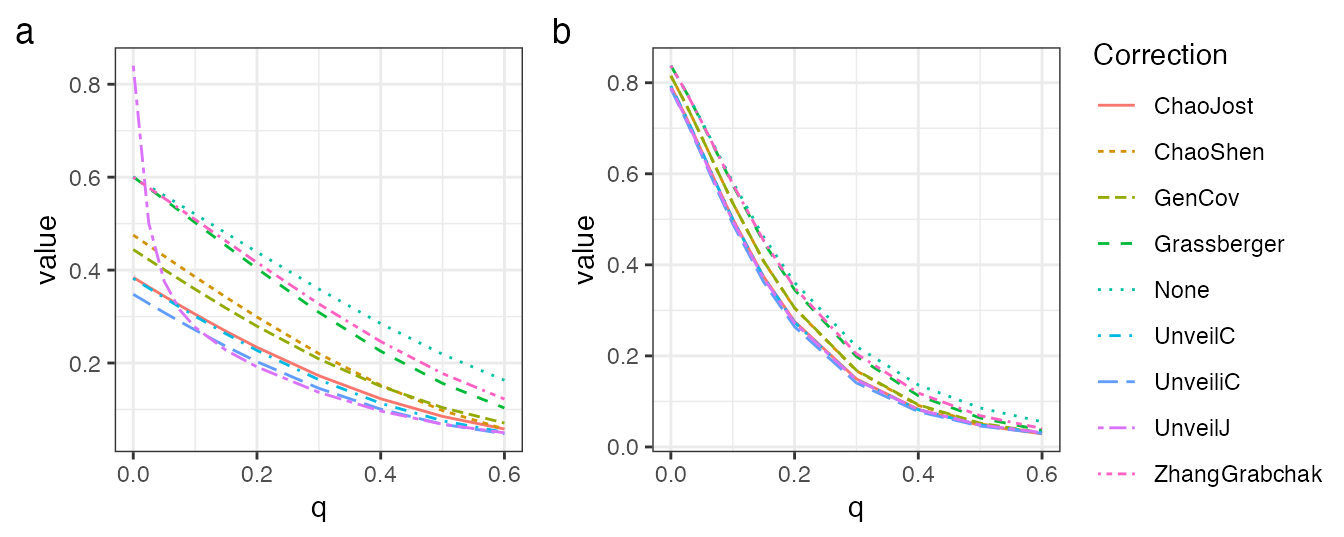
\includegraphics[width=0.8\linewidth]{PracticalEstimation_files/figure-latex/RMSE-1} 

}

\caption{Estimated relative RMSE of the estimators of diversity based on 1000 samples of 1000 individuals of each typical distribution: lognormal (a) and geometric (b) of 300 species. The RMSE is normalized by the actual diversity. It is quite high for low orders of diversity, especially for the geometric distribution. Values of \(q\) over 0.6 are not shown because all estimators perform similarly well. The legend lists the estimators in the increasing order of RMSE for \(q>0.1\), where the estimator with the lowest RMSE is the jackknife-unveiled one, closely followed by the iChao-unveiled and Chao-Jost. Close to \(q=0\), the jackknife-unveiled estimator has a higher variance making it the least reliable estimator.}\label{fig:RMSE}
\end{figure*}

\normalsize

The discussion will focus on the best two estimators: Chao-Jost and jackknife-unveiled, ignoring the iChao-unveiled estimator which takes place between them but is too similar to the jackknife-unveiled to bring decisive arguments for the discussion.
Figure \ref{fig:Profiles} shows their profiles for a 1000-individual sample of a lognormal distribution of 300 species, with their confidence intervals.



\scriptsize

\begin{figure}

{\centering 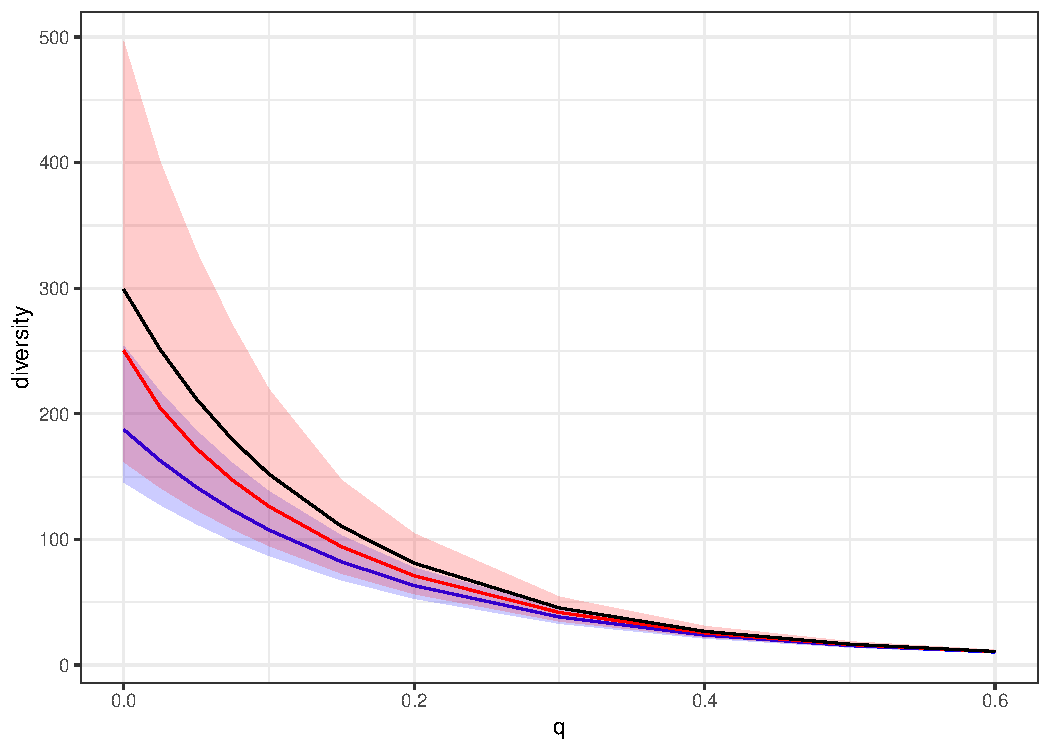
\includegraphics[width=0.8\linewidth]{PracticalEstimation_files/figure-latex/Profiles-1} 

}

\caption{Diversity profiles estimated from 1000 random samples of 1000 individuals from a lognormal community of 300 species. The black line represents the real diversity (starting from \(^{0}{D} \approx 300\)). The jackknife-unveiled estimator is plotted by the red line (\(^{0}{\hat{D}} \approx 250\)). Its confidence interval (red shade) is very wide. The Chao-Jost estimator (blue line: \(^{0}{\hat{D}} \approx 200\)) is more biased downward but its confidence interval (blue shade) is much smaller.}\label{fig:Profiles}
\end{figure}

\normalsize

\hypertarget{discussion}{%
\section{Discussion}\label{discussion}}

The underlying distribution of species is the most important determinant of the success of diversity estimation: the estimation bias of heavy-tailed distributions decays more slowly when the sample size is increased \citep{Zhang2013}.
Estimating the low-order diversity of a sample from a geometric distribution is all but impossible \citep{Haegeman2013} but the low-order diversity of lognormal communities can be estimated meaningfully when the sample size is sufficient.
Empirically, it is not possible to discriminate a severely-censured geometric distribution and a lognormal one \citep{Tokeshi1993}: both models fit well since most of the difference is contained by the unobserved tails of the distributions.
So, theoretical, ecological arguments about the actual distribution of the community are necessary to decide whether an estimation of diversity is reliable.

Diversity of order over 0.5 is pretty well estimated in the context of this paper.
Haegeman \emph{et al.} showed that this remains true for \(q \geq 1\), even when geometric communities of millions of species with parameter 0.5 (the most abundant species takes half the resources, the second one a quarter and so on) are addressed.

\hypertarget{the-sample-coverage-is-not-always-the-good-indicator-of-the-quality-of-estimation}{%
\subsection{The sample coverage is not always the good indicator of the quality of estimation}\label{the-sample-coverage-is-not-always-the-good-indicator-of-the-quality-of-estimation}}

The sample coverage can not be used as a proxy for how much an estimate of diversity can be relied upon.
At the same sampling effort, the sample coverage appears to be higher for the geometric distribution: far more species are not sampled than in a lognormal distribution, but their total probability is smaller.
For example, samples of 200 individuals drawn in 300-species geometric and lognormal communities yield an average estimation of 54 and 149 species by the jackknife-unveiled estimator, but the respective sample coverages are over 95\% for the geometric distribution versus around 81\% for the lognormal one. The estimation bias of the geometric distribution is thus much greater for low orders of diversity even though the sample coverage is higher.

\citet{Chao2012b} argue in favor of the sample coverage as a better measure of the sampling effort than the sample size: this must be understood as long as the underlying distribution of communities is the same.
Then, standardizing the sampling effort by the sample coverage is pertinent.

\hypertarget{comparing-the-diversity-of-real-communities-with-different-distributions-remains-intractable}{%
\subsection{Comparing the diversity of real communities with different distributions remains intractable}\label{comparing-the-diversity-of-real-communities-with-different-distributions-remains-intractable}}

When the number of species of the theoretical distributions is doubled, everything else equal, the sampling bias increases.
With the same sampling effort, the coverage of the lognormal distribution decreases.
Doubling the effort brings both the sample coverage and the bias back to their previous level, with a reduced variance.
These operations can be reproduced with the Shiny application provided with the paper.

This is a very simple and intuitive behavior, but it is completely different with the geometric distribution: the sample coverage does not change when richness is doubled because the probabilities of the 300 rarest species are negligible.
Doubling the sample size does not restore the bias level.
An extensive and rigorous analysis of the influence of the parameters of the theoretical distributions (beyond manipulating the number of species) is not the scope of this paper, but this simple example shows that no general and simple rules are available to compare the low-order diversity of communities of different nature.

\hypertarget{estimating-the-number-of-species-is-the-critical-step}{%
\subsection{Estimating the number of species is the critical step}\label{estimating-the-number-of-species-is-the-critical-step}}

The lower \(q\), the more difficult the estimation is, but the estimation of the number of species has been long studied and simple rules of decision have been proposed \citep{Burnham1979, Brose2003} to choose the most appropriate order of the jackknife estimator.
Burnham and Overton derived a selection procedure to obtain the order allowing to minimize the RMSE of the estimation of the number of species.
It is implemented in the package \emph{SPECIES} {[}\citet{Wang2011}\} for R.
Brose \emph{et al.} showed (empirically) hat the first-order jackknife is selected when the sample completeness \citep[terminology by][]{Beck2010}, i.e.~the proportion of observed species \((S-{s}^{n}_{0})/S\) is over 3/4 (precisely 74\% in their paper).
When it is less, higher orders have less bias but more variance.
It is easy to estimate the number of species of an actual sample this way and compare it to the Chao1 estimator.
If both coincide, the Chao-Jost estimator will perform well for the whole profile: its value at \(q=0\) is that of Chao1.
Else, the jackknife-unveiled estimator will be the best choice since its value at \(q=0\) is the optimal-order jackknife.
If one does not want to rely on the jackknife estimator for some reason, such as its poor theoretical support, the iChao-unveiled estimator is a reasonable compromise as a lower bound estimation.

\hypertarget{better-but-probably-not-much-better-estimators-may-be-derived}{%
\subsection{Better, but probably not much better, estimators may be derived}\label{better-but-probably-not-much-better-estimators-may-be-derived}}

The most promising ways of research according to the present results are a better estimation of the remaining bias of the Zhang-Grabchak estimator and the improvement of the distribution modeling of the unveiled estimators.
The first approach is that of the Chao-Jost estimator, which is limited by its estimation of the number of species (the lower bound, Chao1 estimator).
The price for releasing this constraint is losing the elegant, closed form of the estimator allowed by appropriate approximations of the infinite sum of the unknown elements of eq. \eqref{eq:hq} for a numeric approximation.

The distribution of species is modeled with two parameters in the unveiled estimators.
This can be refined by extending the technique presented by \citet{Chao2014c} to higher orders of sample coverage.
In both cases, better fitting the data to reduce the bias has its limits because the variance of estimation is likely to increase \citep{Bonachela2008}.
So, the estimators presented here may not be far from the optimum trade-off (less bias with the jackknife-unveiled estimator, less variance with Chao-Jost).

\hypertarget{application-to-real-data}{%
\section{Application to real data}\label{application-to-real-data}}



\scriptsize

\begin{figure}

{\centering 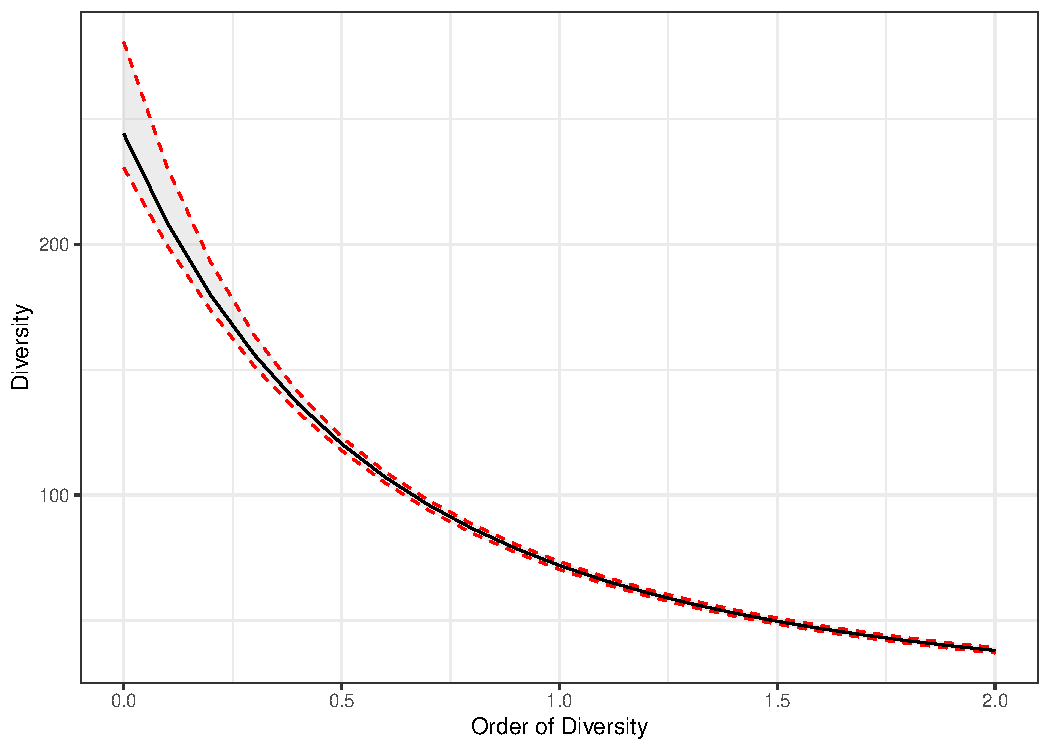
\includegraphics[width=0.8\linewidth]{PracticalEstimation_files/figure-latex/BCIProfile-1} 

}

\caption{Estimated diversity profile of the tree species of the BCI 50-ha plot. The shaded area is the 95\% confidence interval of the estimation.}\label{fig:BCIProfile}
\end{figure}

\normalsize

The diversity of two real forest plots is estimated now.
The first case is Barro Colorado Island's 50-ha plot of tropical forest, whose inventory data of trees over 10\textasciitilde cm diameter at breast height are available in the package \emph{vegan} \citep{Oksanen2012} for R.
225 species have been sampled, with a quite good fit to a lognormal distribution.
The sample size is over 20000 individuals, the sample coverage is over 99.9\%.
Estimating the number of species with the Chao1 or the jackknife 1 estimators gives very similar results: 239 and 244 species.
This is an unusually large dataset, whose diversity estimation (Figure \ref{fig:BCIProfile}) is quite easy.

The best estimator is Chao-Jost since the Chao1 estimator is appropriate for the number of species.
The 95\% confidence interval of the estimation is built by resampling according to the technique by \citet{Chao2015}.
It is very small due to the abundance of data.



\scriptsize

\begin{figure}

{\centering 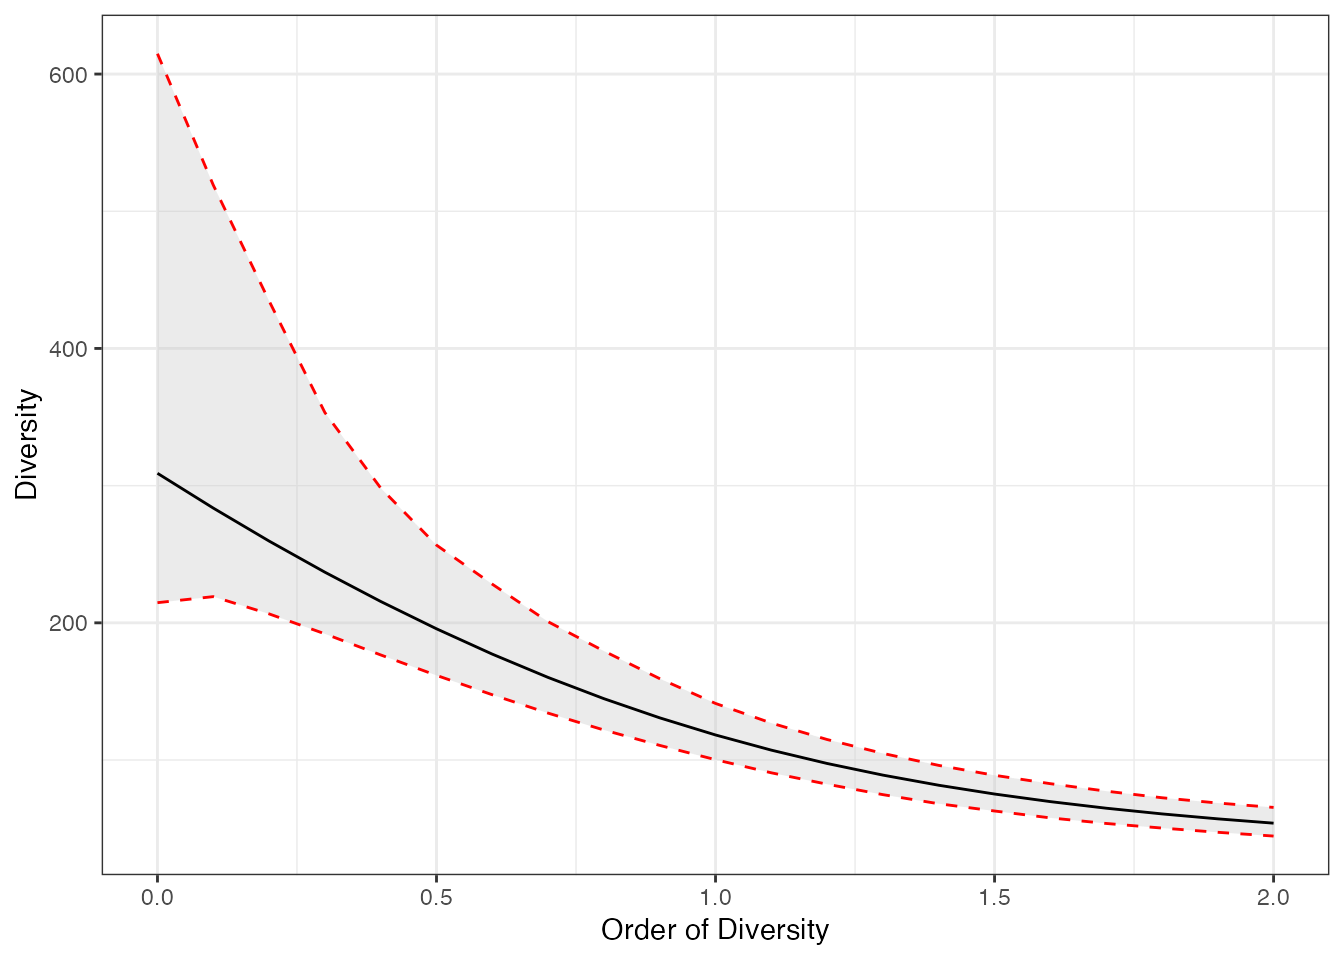
\includegraphics[width=0.8\linewidth]{PracticalEstimation_files/figure-latex/P18Profile-1} 

}

\caption{Estimated diversity profiles of the tree species of the Paracou 1-ha plot \#18. The shaded zone is the 95\% confidence interval of the estimation.}\label{fig:P18Profile}
\end{figure}

\normalsize

The second example takes place at the other extreme of sampling intensity.
A 1-ha plot (plot 18) of tropical forest in the experimental forest of Paracou, French Guiana \citep{Gourlet-Fleury2004}, was inventoried.
Data are available in the package \emph{entropart} for R.
Only 481 trees over 10 cm diameter at breast height have been sampled.
They belong to 149 species.
The sample coverage is \(84.6 \pm 4.4\%\).
The estimated number of species is 254 according to Chao1, but the appropriate Jackknife estimator (of order 3) returns 309 species.
Clearly, the sampling effort is not sufficient for an accurate estimation: the sample coverage is too low and the estimation of the number of species too uncertain.
With no doubt, the Chao-Jost estimator will severely underestimate diversity.

The jackknife-unveiled estimator is the best choice.
Its confidence interval is very wide up to \(q=0.3\) (Figure \ref{fig:P18Profile}).
Over \(q=0.5\), the simulations above showed that the estimator has a very low variability, so the confidence interval is due to the uncertainty of the sampling only.
At lower orders of diversity, the estimator's uncertainty amplifies it so the estimation is not reliable.
In this case, the very little accuracy of the jackknife-unveiled estimator (the number of species is estimated between 237 and 439) is preferable to the far smaller confidence interval provided by a less variable but more biased estimator such as Chao-Jost that would probably not contain the actual values of low-order diversity (as in figure \ref{fig:Profiles}).

\hypertarget{conclusion}{%
\section{Conclusion}\label{conclusion}}

This paper tried to evaluate the performance of diversity estimation in real conditions with simulation studies covering a reasonable set of models.
Unsurprisingly, estimating diversity is more difficult when the species distribution has a heavier tail and the number of species is greater.
As of the state of the art, the recommendation is to apply the Chao-Jost, the iChao-unveiled or the jackknife-unveiled estimator and consider diversity of order lower than 0.5 with caution.

When the sampling effort is high enough to allow a correct estimation of the number of species with the Chao1 estimator, the estimation by Chao-Jost is quite good down to \(q=0\).
If this is not the case, the jackknife-unveiled estimator provides better results but with a higher variability.
A conservative compromise for a first estimation of diversity, before choosing between Chao-Jost and jackknife-unveiled, is the iChao-unveiled estimator.

The \emph{entropart} package for R allows computing species-neutral diversity and phylodiversity with all the estimators presented here.

\hypertarget{acknowledgments}{%
\section{Acknowledgments}\label{acknowledgments}}

This work has benefited from an ``Investissement d'Avenir'' grant managed by Agence Nationale de la Recherche (CEBA, ref. ANR-10-LABX-25-01).

%----------------------------------------------------------------------------------------
%	REFERENCE LIST
%----------------------------------------------------------------------------------------

\bibliographystyle{chicago}
\makeatletter
% The filename has .bib extension that must be eliminated
\filename@parse{references.bib}
% parse stores the file name in base. Extension starts at the first dot, so don't use dots in file names.
\bibliography{\filename@base}
\makeatother


%----------------------------------------------------------------------------------------

\end{document}
